\documentclass{beamer}

%% \documentclass[handout]{beamer}
%% % use this with the [handout] option to create handouts for the audience
%% \usepackage{pgfpages}
%% \pgfpagesuselayout{2 on 1}[a4paper,border shrink=5mm]

\mode<presentation>
{
  \usetheme{Diku}
% set this to your preferences:
%  \setbeamercovered{invisible}
  \setbeamercovered{transparent}
}

\usepackage{graphicx}
\usepackage{epic}

\usepackage{amsmath}
\usepackage{amssymb}
\usepackage{amsthm}

\usepackage{minibox}
\usepackage{listings}
\newcommand{\basetop}[1]{\vtop{\vskip-1ex\hbox{#1}}}
\newcommand{\source}[1]{\let\thefootnote\relax\footnotetext{\scriptsize\textcolor{kugray1}{Source: #1}}}

% for coloured code citation in text:
\usepackage{fancyvrb}

%%%%%%%%%%%%%%%%%%%%%%%%%%%%%%%%%
%%%%%    code sections   %%%%%%%%
%%%%%%%%%%%%%%%%%%%%%%%%%%%%%%%%%

% code highlighting commands in own block
\DefineVerbatimEnvironment{code}{Verbatim}{fontsize=\scriptsize}
\DefineVerbatimEnvironment{icode}{Verbatim}{fontsize=\scriptsize}

% Fancy code with color commands:
\DefineVerbatimEnvironment{colorcode}%
        {Verbatim}{fontsize=\scriptsize,commandchars=\\\{\}}

%%%%%%%%%%%%%%%%%%%%%%%%%%%%%%%%%%
%%%%%    some coloring    %%%%%%%%

\definecolor{Red}{RGB}{220,50,10}
\definecolor{Blue}{RGB}{0,51,102}
\definecolor{Yellow}{RGB}{102,51,0}
\definecolor{Orange}{RGB}{178,36,36}
\definecolor{Grey}{RGB}{180,180,180}
\definecolor{Green}{RGB}{20,120,20}
\definecolor{Purple}{RGB}{160,50,100}
\newcommand{\red}[1]{\textcolor{Red}{{#1}}}
\newcommand{\blue}[1]{\textcolor{Blue}{{#1}}}
\newcommand{\yellow}[1]{\textcolor{Yellow}{{#1}}}
\newcommand{\orange}[1]{\textcolor{Orange}{{#1}}}
\newcommand{\grey}[1]{\textcolor{Grey}{{#1}}}
\newcommand{\green}[1]{\textcolor{Green}{{#1}}}
\newcommand{\purple}[1]{\textcolor{Purple}{{#1}}}



% use "DIKU green" from our color theme for \emph
\renewcommand{\emph}[1]{\textcolor{structure}{#1}}
% use some not-too-bright red for an \emp command
\definecolor{DikuRed}{RGB}{130,50,32}
\newcommand{\emp}[1]{\textcolor{DikuRed}{ #1}}
\definecolor{CosGreen}{RGB}{10,100,70}
\newcommand{\emphh}[1]{\textcolor{CosGreen}{ #1}}
\definecolor{CosBlue}{RGB}{55,111,122}
\newcommand{\emphb}[1]{\textcolor{CosBlue}{ #1}}
\definecolor{CosRed}{RGB}{253,1,1}
\newcommand{\empr}[1]{\textcolor{CosRed}{ #1}}

\newcommand{\mymath}[1]{$ #1 $}
\newcommand{\myindx}[1]{_{#1}}
\newcommand{\myindu}[1]{^{#1}}
\newcommand{\mymathbb}[1]{\mathbb{#1}}


\newtheorem{mydef}{Definition}
\newtheorem{mytheo}{Theorem}
\newtheorem{mylemma}{Lemma}

\newcommand{\Fn}{\ensuremath{\lambda}}

\lstdefinelanguage{Futhark}
{keywords={fun,if,then,else,loop,do,map,reduce,filter,scan,redomap,transpose,rearrange,reshape,iota,replicate,let,in,for,while,with,f32,i32,i8,u8,zip,stream_red,unsafe,local},%
  sensitive=true,%
  comment=[l]{--},%
  string=[b]",%
  literate={\\}{\Fn}{1} {->}{$\rightarrow$}{1} {<-}{$\leftarrow$}{1},
  moredelim=**[is][\color{red}]{@}{@},
  moredelim=**[is][\color{blue}]{!}{!},
}

\lstdefinelanguage{none}{
  identifierstyle=
}

\lstset{
  language=Futhark,
  basicstyle=\footnotesize
}


%%%%%%%%%%%%%%%%%%%%

%Non-Heroic AutoPar
\title[]{A Quick Study of Data Parallelism in\\
        Imperative {\em vs.} Functional Languages}

%C.~Oancea
\author[]{Cosmin E. Oancea\\{\tt cosmin.oancea@diku.dk}}

\institute{Department of Computer Science (DIKU)\\University of Copenhagen}


\date[23/11/2017]{23rd of November 2017}


\begin{document}

\titleslide

\begin{frame}[fragile]
	\tableofcontents
\end{frame}


\section{Automatic Parallelization for Fortran77-like Languages}

\begin{frame}[fragile,t]
  \frametitle{Imperative Approaches}

\begin{itemize}
    \item \emphh{Perspective:}
        automatic parallelization of loop-based sequential code 
        in mainstream languages $\Rightarrow$ highest impact
    \bigskip 

    \item \emphh{Restrictive or Heroic Analysis:}
        \begin{itemize}
            \item assumes (morally) Fortran77 code;            
            \item fights the language (aliasing, 
                    indirect accesses, control flow);
            \item low-level data-dependency analysis
                    (of array indices inside loops); 
            \item reverse engineers user's sequential
                    optimizations.
            %\item reverse engineers user's sequential optimizations
        \end{itemize}
    \bigskip

    \item \emphh{Guarantees:} none!\\
        ``What happens when you try a new benchmark?''
    \bigskip
\end{itemize}

\end{frame}

\begin{frame}[fragile,t]
  \frametitle{Definition of a Data Dependency} % of CPU, Multicores, GPGPU
\vspace{-2ex}
\begin{block}{Load-Store Classification of Dependencies}
\begin{colorcode}
True Dependency (RAW)    Anti Dependency (WAR)    Output dependency (WAW)
S1    X  = ..            S1    .. = X             S1    X = ...            
S2    .. = X             S2    X  = ..            S2    X = ...
\end{colorcode}
\end{block} 
\pause
\bigskip

{\bf Def. Loop Dependence:} There is a dependence from statement $S1$ to $S2$
in a loop nest {\em iff} $\exists$ iterations $\vec{k}$, $\vec{l}$ such that:
\begin{description}
    \item[1.] $\vec{k} < \vec{l}$ or $\vec{k} = \vec{l}$ and $\exists$ 
                an execution path from statement $S1$ to statement $S2$ \emp{such that:}
    \item[2.] $S1$ accesses memory location $M$ on iteration $\vec{k}$, and
    \item[3.] $S2$ accesses memory location $M$ on iteration $\vec{l}$, and
    \item[4.] one of these accesses is a write.
\end{description}
\medskip

%\emp{We say that $S1$ is the source and $S2$ is the sink of the dependence}, 
%because $S1$ executes before $S2$ in the sequential program execution.
%Dependence depicted with an arrow pointing from source to sink.\pause

\end{frame}

\begin{frame}[fragile,t]
  \frametitle{Intuition: Dependence Analysis of Loops}

\blue{Analysis of array subscripts aims at disproving dependencies across loop iterations, 
i.e., $\vec{k} < \vec{l}$. Two directions:}\medskip
\begin{itemize}
    \item[1] analyse each pair of read/write-write accesses (polyhedral)
        \begin{itemize}
               \item accurate under affine indexing and control flow.\medskip
        \end{itemize}

    \item[2] summarize memory references $+$ model parallelism as an equation 
                on abstract sets $+$ extract sufficient conditions 
            \begin{itemize}
               \item more suitable for larger, non-affine loops \medskip
            \end{itemize}
\end{itemize}

\begin{block}{ Loop Eg.{\tt~~~~~~~~~~~~}Pointwise RAW{\tt~~~~}Summarization RAW} \vspace{-1ex}
\begin{columns}
\column{0.20\textwidth}
\begin{colorcode}[fontsize=\scriptsize]
DO \emph{i = 1, N}
  A(\emp{i+100}) = ..
  IF x>0 THEN
    ... = A(\emp{i})
  ENDIF
ENDDO
\end{colorcode}
\column{0.21\textwidth}
\begin{colorcode}[fontsize=\scriptsize]
\emph{1\mymath{\leq}i\mymath{\myindx{1}\leq}N}
\emph{1\mymath{\leq}i\mymath{\myindx{2}\leq}N}
\emp{i\mymath{\myindx{1}}+100 \mymath{=} i\mymath{\myindx{2}}}

NOT PARALLEL 
\mymath{\Leftrightarrow} \mymath{\exists} sol i\mymath{\myindx{1}\neq}i\mymath{\myindx{2}}
\end{colorcode}
%\column{0.21\textwidth}
%\begin{colorcode}[fontsize=\scriptsize]
%\mymath{\lceil}READ \mymath{\rceil}=[1,N]
%\mymath{\lceil}WRITE\mymath{\rceil}=[101,N+100]
%
%\mymath{\lceil}READ\mymath{\rceil}\mymath{\cap}\mymath{\lceil}WRITE\mymath{\rceil} = \mymath{\emptyset}
%\mymath{\Rightarrow} (N \mymath{\geq} 100)
%\mymath{\Rightarrow} PARALLEL
%\end{colorcode}
\column{0.30\textwidth} 
\begin{center} \hspace{-4ex}
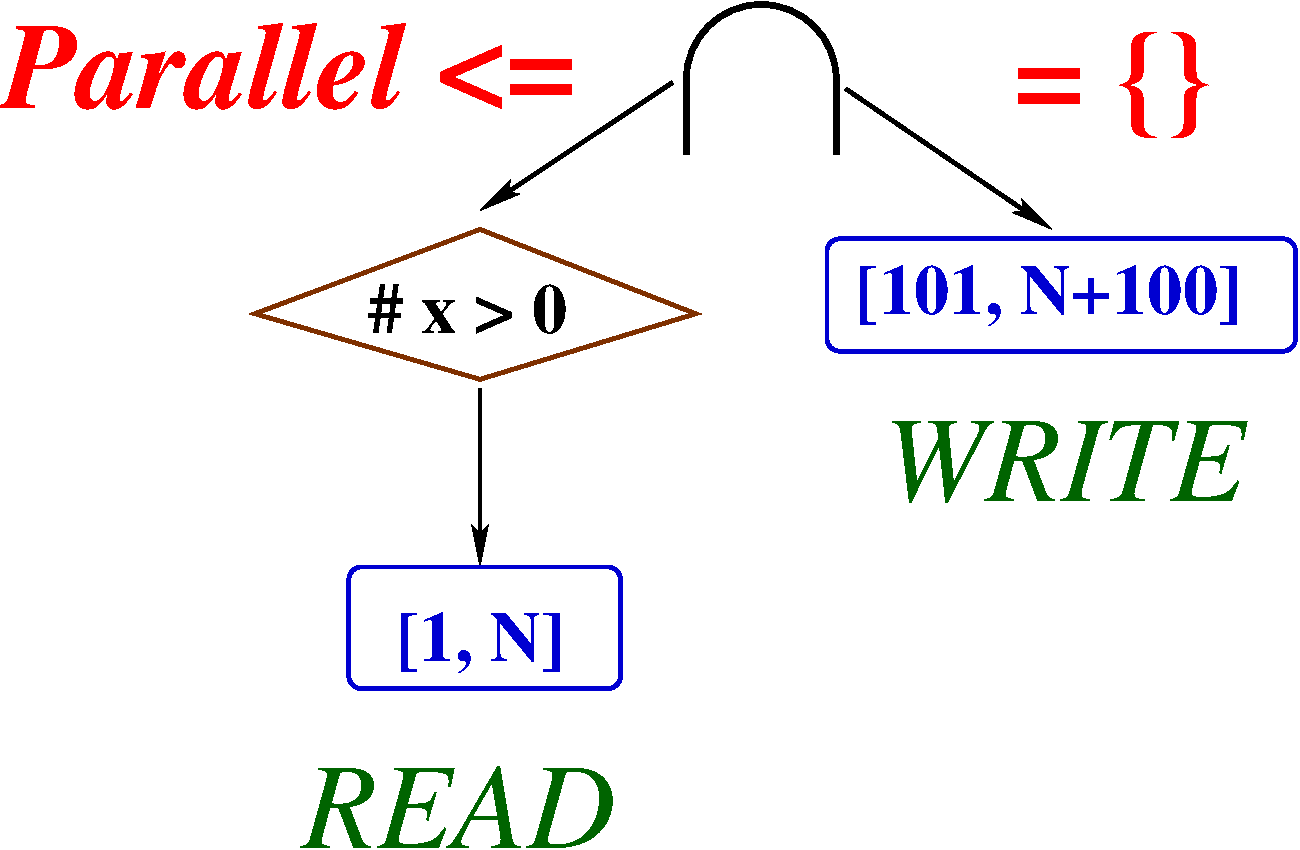
\includegraphics[height=13ex]{Figures/SimpleInd}
\end{center}
\end{columns}
\end{block}
 


%1. Unified Set Reference (USR) [Rus,Rauchwerger,Hoeflinger,2003].\\
%2. Extract a sufficient condition for parallelism, in our case
%{\tt $x\leq 0$~$\vee$~$N \leq 100$} \mymath{\Rightarrow} PARALLEL

Sufficient condition for parallelism: {\tt $x\leq 0$~$\vee$~$N \leq 100$} \mymath{\Rightarrow} PARALLEL.

\end{frame}


\begin{frame}[fragile,t]
  \frametitle{Motivation for Hybrid (static + dynamic) Analysis}

\begin{block}{Approach Centered on Extracting Arbitrarily Shaped Predicates:} 
\begin{columns}
\column{0.25\textwidth}
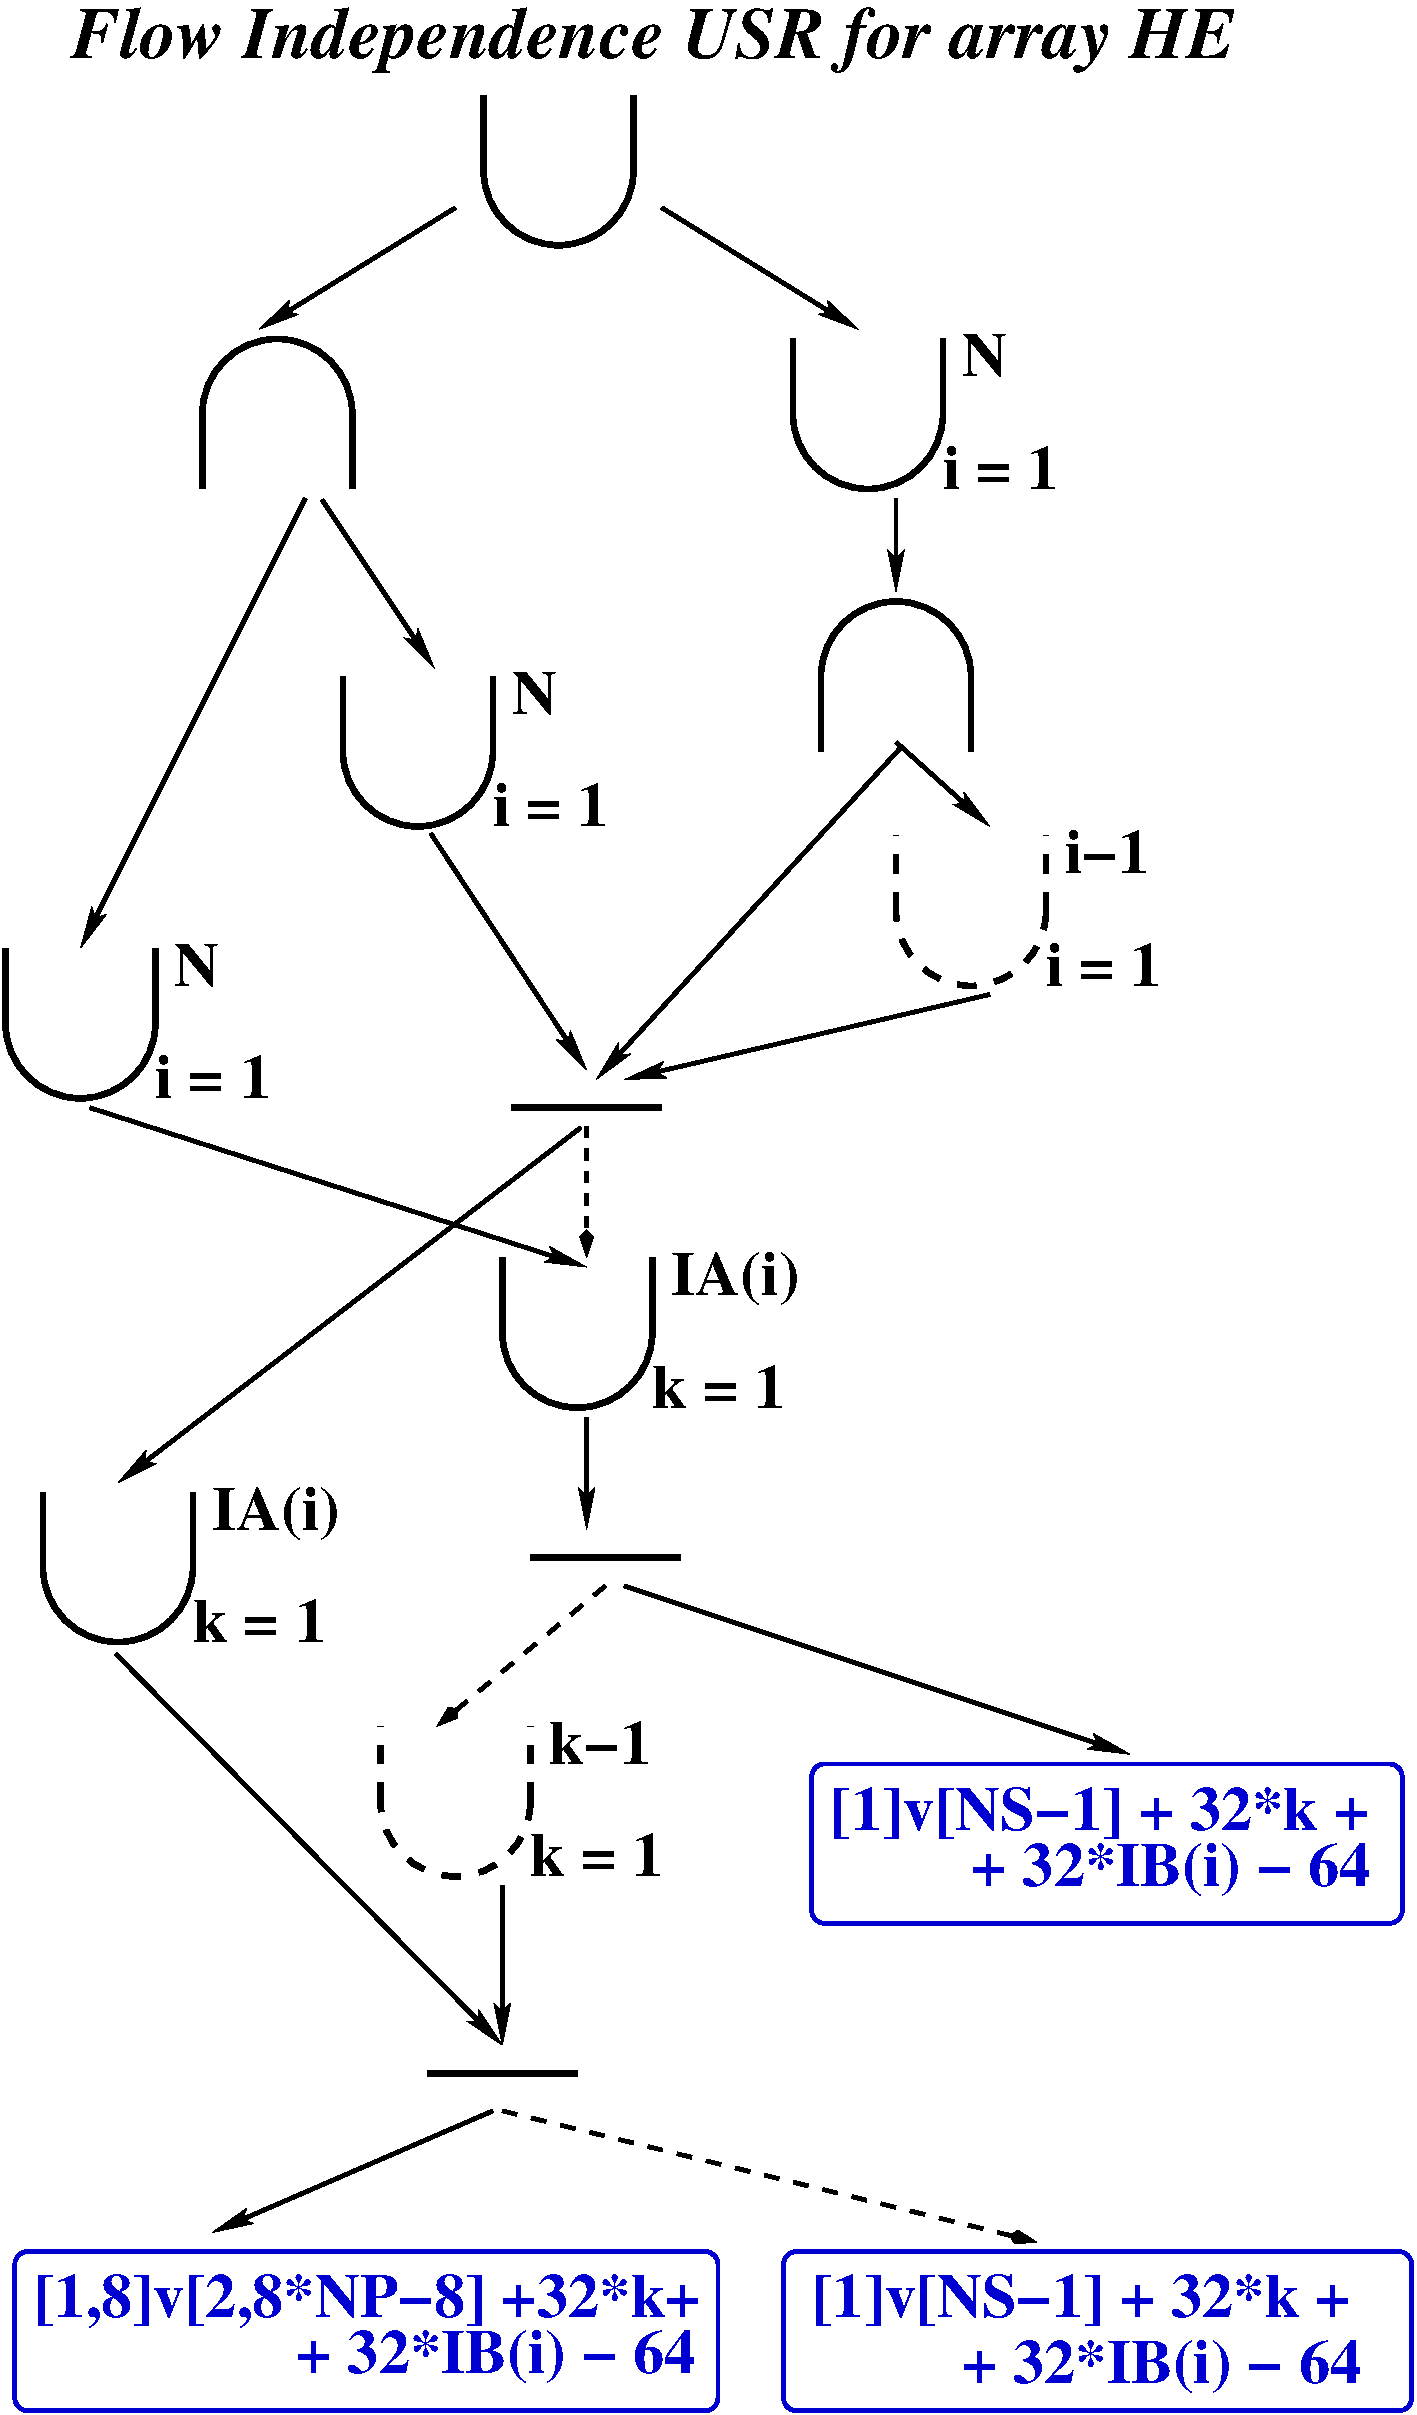
\includegraphics[height=28ex]{Figures/USR_HE_FIND_SOLVH}
\column{0.73\textwidth}\vspace{-1ex}
\begin{itemize}
    \item \emp{\em Proof of parallelism: often dataset sensitive.}\medskip
    \item \emp{{\em Source of inaccuracy:}} summary repres not closed under composition w.r.t. set operations, leads to early conservative approx.\medskip
    \item \emph{{\em Language}} representation for summaries ... precise but \emp{expensive} to compute at runtime \medskip
    \item ``Let's \emph{{\em reason}} about it!'' $S=\emptyset$ $\Leftarrow$ $\emp{A - B} = \emptyset \Leftarrow$ \emph{$8*NP < NS + 6$}!
\end{itemize}
\end{columns}
\end{block}


%{\tiny S.~Rus, L.~Rauchwerger and J.~Hoeflinger, ``Hybrid analysis: static \& dynamic memory reference analysis'', IJPP'03.}\\
{\tiny C.~E.~Oancea and L.~Rauchwerger, ''A Hybrid Approach to Proving Memory Reference Monotonicity'', LCPC'11.}\\
{\tiny C.~E.~Oancea and L.~Rauchwerger, ''Logical Inference Techniques for Loop Parallelization'', PLDI'12.}\\
{\tiny C.~E.~Oancea and L.~Rauchwerger, ''Scalable Conditional Induction Variable (CIV) Analysis'', CGO'15.}

\end{frame}


\begin{frame}[fragile,t]
  \frametitle{Main Steps in Hybrid (static + dynamic) Analysis}
%  \frametitle{Paper's Approach Overview}

Extraction of arbitrary predicates of ``quasi-optimal'' complexity:
%that prove loop independence.
\begin{itemize}

    \item \emph{{\em Language}} to represent summaries: use $-, \cap, \cup_{i=1}^N$, gate, callsite
            nodes when operations fall outside the array-abstraction domain.\smallskip
    
    \item \emph{{\em Translate}} to a language of predicates ($\wedge_{i=1}^{N}, \vee$) \\
            $\mbox{ }\mbox{ }\mbox{ }\mbox{ }\mbox{ }\mbox{ }\mbox{ }$
                \emph{$\mathcal{F} : Summary \rightarrow Predicate$  $\mbox{ }\mbox{ }\mbox{ }$ 
                $S = \emptyset \mbox{ }\Leftarrow\mbox{ }\mathcal{F}(S)$}. \smallskip

    \item The result is factorized into a cascade of predicates, which are \\
            tested at runtime in the order of their estimated complexity. \smallskip

\end{itemize}


{\tiny S.~Rus, L.~Rauchwerger and J.~Hoeflinger, ``Hybrid analysis: static \& dynamic memory reference analysis'', IJPP'03.}\\\smallskip
{\tiny C.~E.~Oancea and L.~Rauchwerger, ''A Hybrid Approach to Proving Memory Reference Monotonicity'', LCPC'11.}\\\smallskip
{\tiny C.~E.~Oancea and L.~Rauchwerger, ''Logical Inference Techniques for Loop Parallelization'', PLDI'12.}\\\smallskip
{\tiny C.~E.~Oancea and L.~Rauchwerger, ''Scalable Conditional Induction Variable (CIV) Analysis'', CGO'15.}\\\smallskip

\end{frame}


\begin{frame}[fragile,t]
  \frametitle{Experimental Results: Perfect-Club \& SPEC Bench} \vspace{-1ex}
\begin{columns} 
\column{0.48\textwidth} 
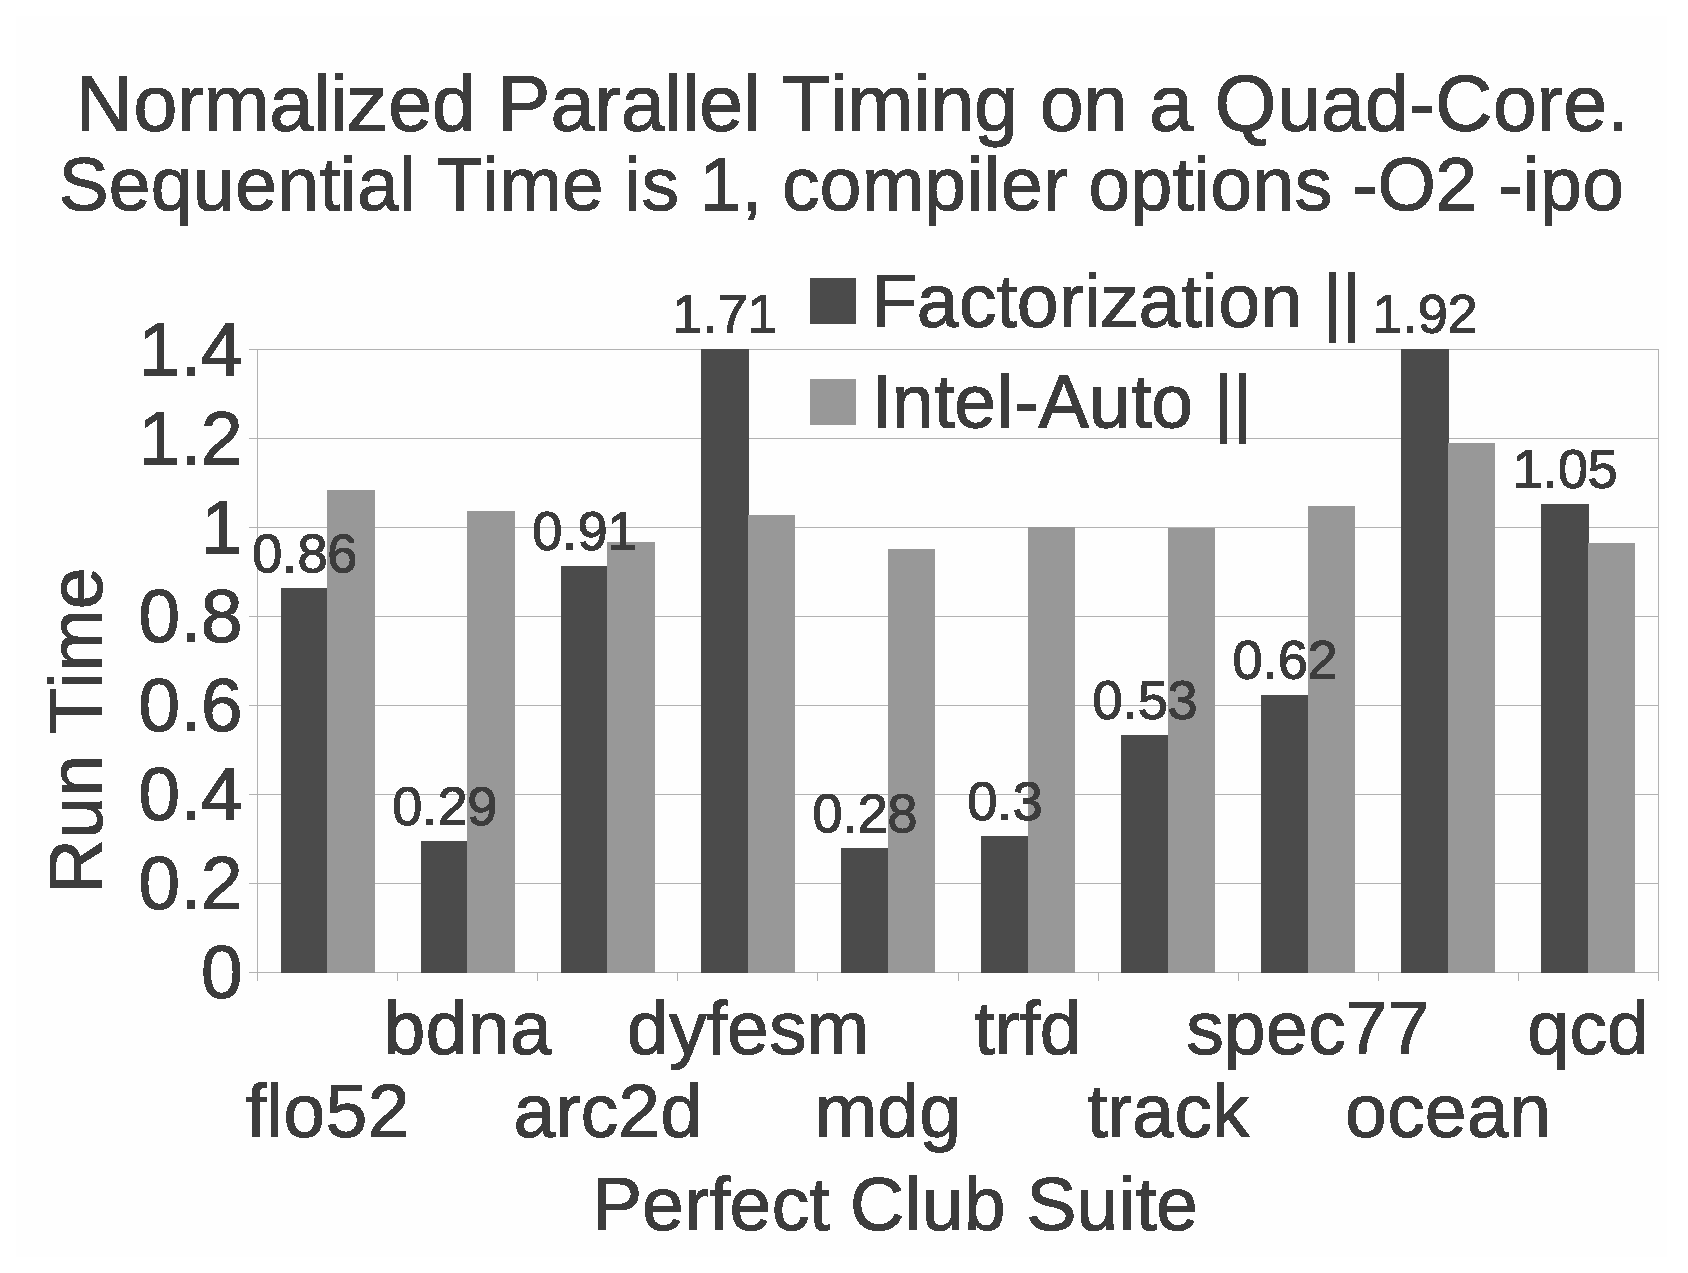
\includegraphics[height=22ex]{Figures/PerfectResO2}
\column{0.48\textwidth} 
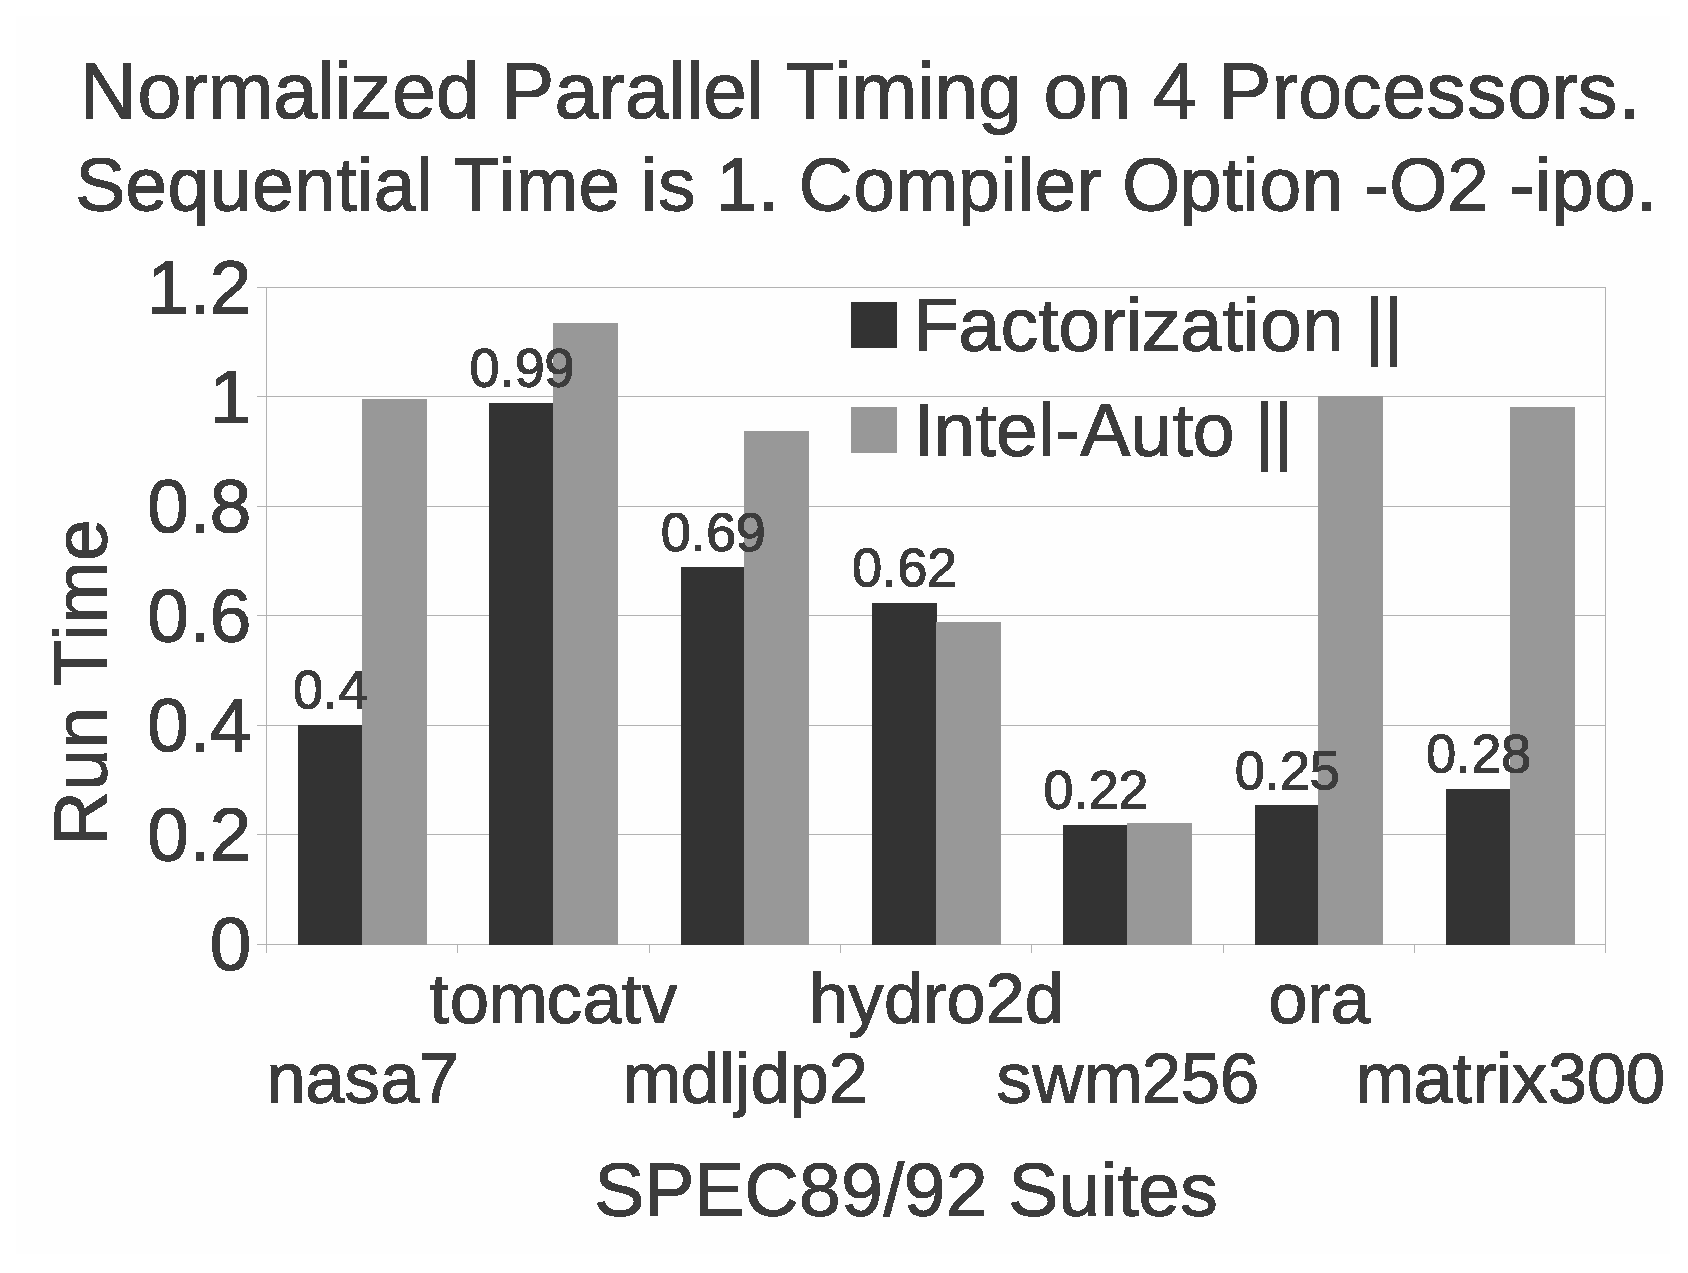
\includegraphics[height=22ex]{Figures/Spec92ResO2}
\end{columns}
%\smallskip
\begin{columns} 
\column{0.48\textwidth} 
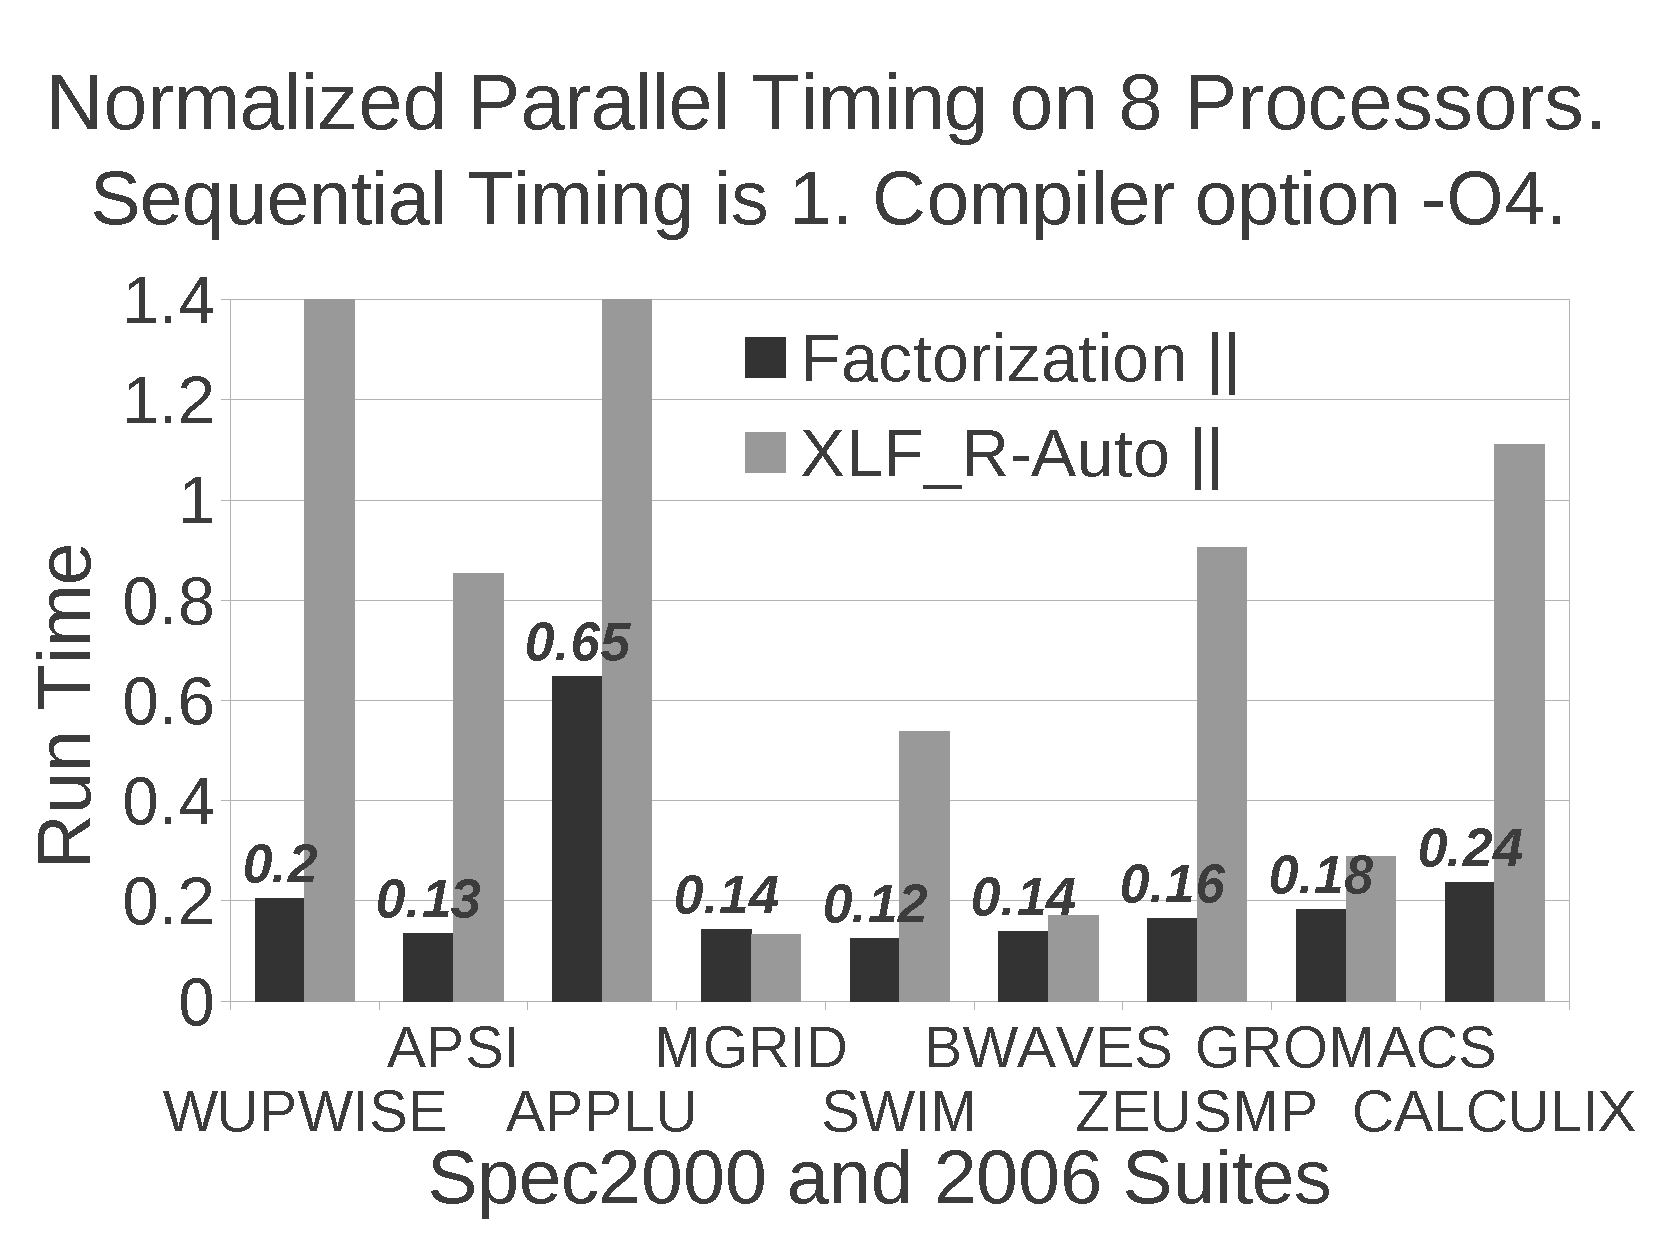
\includegraphics[height=25ex]{Figures/Spec2006Res}
\column{0.48\textwidth} 
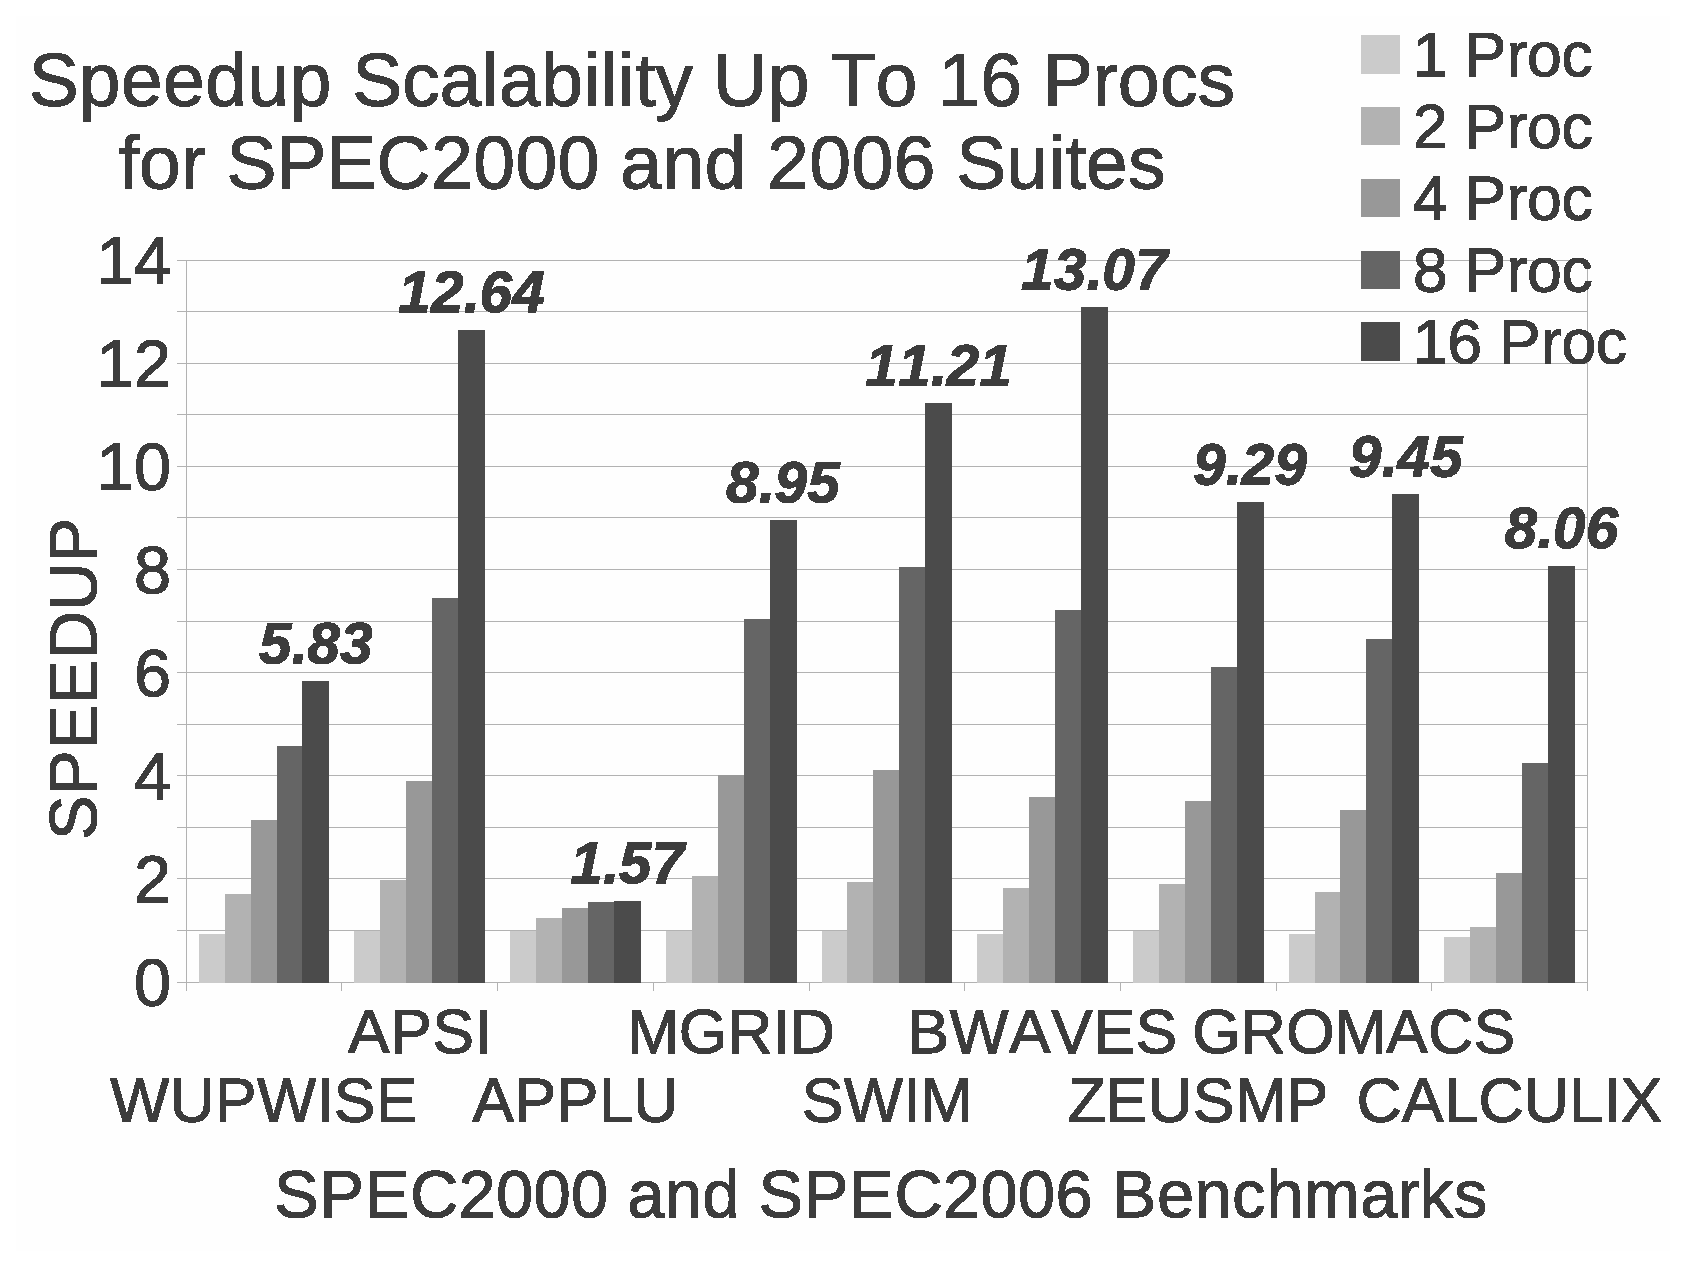
\includegraphics[height=25ex]{Figures/Spec2006SpeedupScalRTall}
\end{columns}

\end{frame}


\begin{frame}[fragile,t]
  \frametitle{Evaluation on $30$ {\sc perfect-club} \& {\sc spec} benches}
%  \frametitle{Paper's Approach Overview}

\emph{Analysis Is Effective in Most Cases:}\smallskip
\begin{itemize}
                \item Analyzed $2100$ loops, measured $380$ parallel loops $92\%$ runtime,\smallskip
                \item \emph{Good application-level speedup at negligible predicate overhead};
                        not pretty but effective, e.g., {\tt mafillsm\_do7} in {\scriptsize \textsc{Calculix}/\textsc{Spec2006}},\smallskip 
                \item \emph{Only 2 loops} out of 380, i.e., $\sim0.5\%$, \emph{require {\sc tls}}.
\end{itemize}

\bigskip
\pause
\emp{Sill a Heroic-Effort Solution:}\smallskip
\begin{itemize}
                \item \emp{Complex Analysis}: 2 {\em helper} {\sc ir}s \& optims, complex codegen\smallskip
                \item \emp{Compiler Magic}: parallelism may {\em not} be discovered, {\scriptsize 416.gamess}, 
                \item \emp{Main Difficulty}: user's optimizations obfuscates parallelism \& 
                  reverse engineering them is hard, e.g., {\tt scan} (prefix sum).\smallskip
                \item \emp{\bf Unsuitable to build on it}, e.g., nested parallelism, locality. 
                \medskip
\end{itemize}

%\alert{Obs:} Summary, Predicate, and SSA reps are pure functional langs!

{\tiny
%S.~Rus, L.~Rauchwerger and J.~Hoeflinger, ``Hybrid analysis: static \& dynamic memory reference analysis'', IJPP'03.
C.~E.~Oancea and L.~Rauchwerger, ''A Hybrid Approach to Proving Memory Reference Monotonicity'', LCPC'11.
C.~E.~Oancea and L.~Rauchwerger, ''Logical Inference Techniques for Loop Parallelization'', PLDI'12.$\mbox{\tt~~~~~~}$
C.~E.~Oancea and L.~Rauchwerger, ''Scalable Conditional Induction Variable (CIV) Analysis'', CGO'15.
}

%\includegraphics[height=7ex]{Figures/IND_PRED/indequ.ps}
%\includegraphics[height=7ex]{Figures/IND_PRED/pred_big.ps}
%\includegraphics[height=7ex]{Figures/IND_PRED/pred_o1.ps}

\end{frame}


\section{Explicit Parallelism in Data-Parallel (Functional) Languages}

\begin{frame}[fragile]
	\tableofcontents[currentsection]
\end{frame}

\begin{frame}[fragile,t]
   \frametitle{Data-Parallel Purely-Functional Language}

\blue{\em Language designed to help the compiler:}\bigskip
\begin{itemize}
    \item[+] \emphh{explicit parallelism} by means of bulk-parallel operators\\ 
                promoting higher order semantics + race-free guarantees;\bigskip
    \item[+] easier to reason when:
        \begin{itemize}
            \item functions are math functions,
            \item no destructive updates;
        \end{itemize}\bigskip
    \item[+] \emphh{flattening}: general transformation of nested parallelism into
                flat parallelism preserving work and depth asymptotics;\bigskip
    \item[-] \emp{often inefficient;}\bigskip
    \item[-] \emp{require a learning curve}, i.e., not general purpose/mainstream.\bigskip
\end{itemize}

\end{frame}

\begin{frame}[fragile,t]
   \frametitle{Data-Parallel Functional Language}

\emp{map} :: $((\alpha \rightarrow \beta), [n]\alpha) \rightarrow [n]\beta $ has \emph{\em inherently parallel semantics}.

\bigskip

\begin{tabular}{crcccccl}
x = & \emp{map}(~~~f, \{& $a_1$, & $a_2$, & .., & $a_n$ & \} & )\\
    &      & $\downarrow$ & $\downarrow$ &  & $\downarrow$ & &\\
x $\equiv$ &  \{  & \emph{f($a_1$)}, & \emph{f($a_2$)}, & .., & \emph{f($a_n$)} & \} &
\end{tabular}

\bigskip
\bigskip
\pause

\emp{Map Fusion:} (higher-order transformation)

\begin{tabular}{rccc}
a = & \{ $a_1$, $a_2$, .., $a_n$ \} & & a = \{ $a_1$, $a_2$, .., $a_n$ \} \\  
\emp{x =} & \emp{map( f, a )} & & \\
%  & $\downarrow$ & & \\
%//x = &  \{ \emph{f($a_1$)}, \emph{f($a_2$)}, .., \emph{f($a_n$)} \} & & \\
\emph{y} = & \emp{map( g, x )} & $\equiv$ & \emph{y} = \emp{map(g o f, a)}\\
  & $\downarrow$ & & \\
\emph{y} $\equiv$ &  \{\emph{g(f($a_1$))},\emph{g(f($a_2$))},..,\emph{g(f($a_n$))}\} & $\equiv$ & \{\emph{g(f($a_1$))},\emph{g(f($a_2$))},..,\emph{g(f($a_n$))}\} \\
\end{tabular}

\end{frame}


\begin{frame}[fragile,t]
   \frametitle{Map-Reduce Functional Language}

\bigskip

\emp{reduce} :: $((\alpha \rightarrow \alpha \rightarrow \alpha), \alpha, []\alpha) \rightarrow \alpha$

\smallskip

\emp{reduce}($\odot$, $e$, \{$a_1$, $a_2$, ..., $a_n$\}) $\equiv$ \emph{$e \odot a_1 \odot a_2 \odot ... \odot a_n$}

\smallskip

~~~~~where $\odot$ is an associative binary operator.

\bigskip

\begin{center} 
        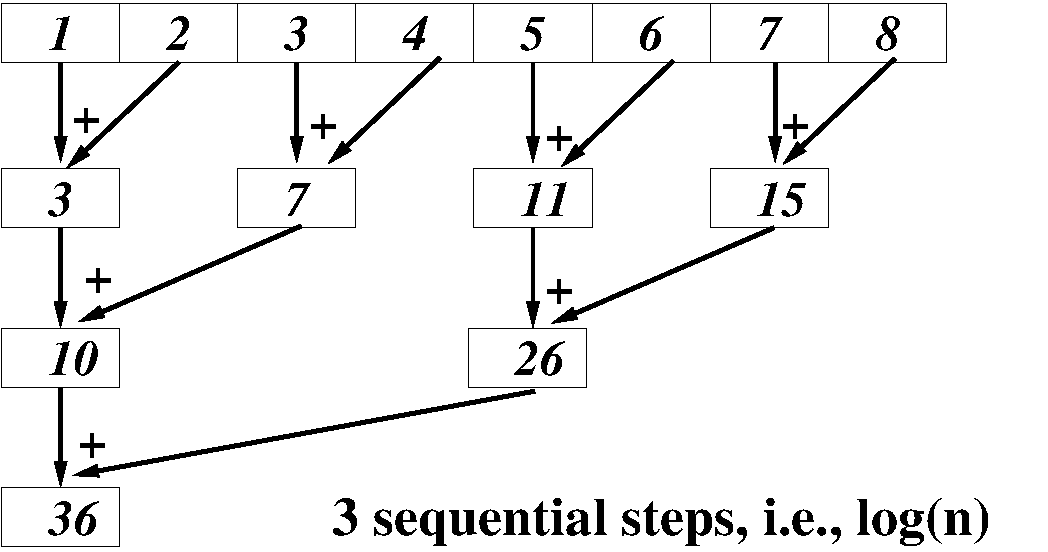
\includegraphics[height=18ex]{Figures/ReduceEg.pdf} 
\end{center}\bigskip


\blue{Build programs by nested composition of such parallel operators}\\
(\emp{map}, \emp{reduce}, etc.)

\end{frame}

\section{Current and Future Research}

\begin{frame}
  \begin{center}
    \Huge
    Current and\\
    Future Research
  \end{center}
\end{frame}


\subsection{Futhark: Common Ground Between Functional and Imperative}

%\begin{frame}[fragile]
%	\tableofcontents[currentsection]
%\end{frame}

\begin{frame}
  \frametitle{Futhark: Motivation}

\emp{Weaknesses of purely-functional data-parallel languages:}
\begin{itemize}
    \item[-] do not support dependent loops with in-place updates;
    \item[-] preserving asymptotics often sacrifices the common case 
        \begin{itemize}
            \item application parallelism not tuned to hardware,
            \item full flattening prevents locality optimisations.
        \end{itemize}
\end{itemize}
\bigskip

\emphh{Futhark: common ground combining the advantages}
\begin{itemize}
    \item[+] supports a restrictive notion of in-place updates (and loops)
    \item[+] models high-impact imperative optimizations by higher-order reasoning:
        \begin{itemize}
            \item efficient sequentialization of parallelism in excess;
            \item partial flattening builds on loop distribution/interchange,\\ 
                    and allows further locality optimizations.
        \end{itemize}
\end{itemize}
\medskip

\tiny{
C.~Andreetta, V.~Bégot, J.~Berthold, M.~Elsman, F.~Henglein, T.~Henriksen, M.~B.~Nordfangand, and C.~E.~Oancea. ``Finpar: A parallel financial benchmark'', TACO'16.\\
T~Henriksen, M.~Elsman, F.~Henglein, and C.~E.~Oancea. ``Futhark: purely functional GPU-programming with nested parallelism and in-place array updates'', PLDI'17.
}

\end{frame}


\begin{frame}[fragile,t]
  \frametitle{Tunable Parallelism: k-Means/Histogram Example}

\emp{Completely sequential} and \emphh{work efficient:}
\begin{lstlisting}
let counts = 
  loop (counts = replicate k 0) for i < n do
    let cluster = membership[i]
    let counts[cluster] = counts[cluster] + 1
    in  counts
\end{lstlisting}
\bigskip
\pause

\emphh{Completely parallel} and \emp{work inefficient:}
\begin{lstlisting}
let increments =
     map(\(cluster: int): [k]int ->
              let incr = replicate k 0
              let incr[cluster] = 1 
              in  incr
        ) membership
let counts = reduce (map (+)) (replicate k 0) increments
\end{lstlisting}
\end{frame}

\begin{frame}[fragile,t]
  \frametitle{Tunable Parallelism: k-Means/Histogram Example}

\emphh{Just Right:}
\begin{lstlisting}
let counts = 
      stream_red (map (+))
                 (\ (chunk: [!chunksize!]int): [k]int ->
                    loop (acc = replicate k 0) 
                      for i < !chunksize! do
                        let cluster = chunk[i]
                        let acc[cluster] = acc[cluster]+1
                        in  acc
                 )
                 (replicate k 0) 
                 membership
\end{lstlisting}

\smallskip

\tiny{
C.~Andreetta, V.~Bégot, J.~Berthold, M.~Elsman, F.~Henglein, T.~Henriksen, M.~B.~Nordfangand, and C.~E.~Oancea. ``Finpar: A parallel financial benchmark'', TACO'16.\\$\mbox{ }$\\
T~Henriksen, M.~Elsman, F.~Henglein, and C.~E.~Oancea. ``Futhark: purely functional GPU-programming with nested parallelism and in-place array updates'', PLDI'17.
}

\end{frame}

\begin{frame}
  \frametitle{Speedup Over Hand-Written Rodinia OpenCL Code on NVIDIA GTX780 Ti and AMD W8100 GPUs}

  \begin{center}
    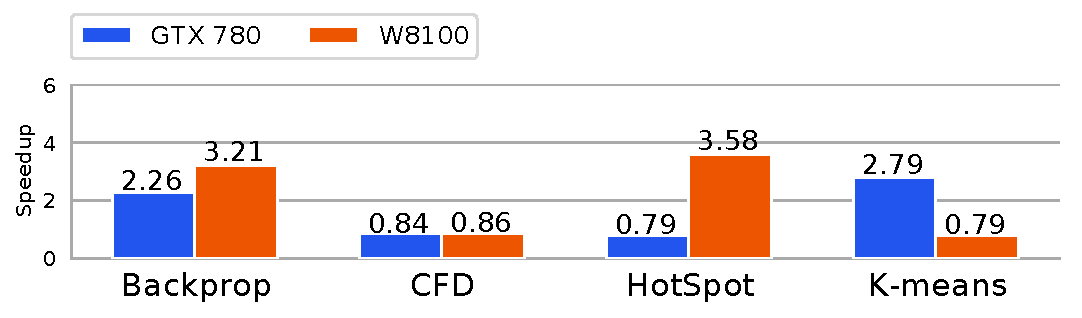
\includegraphics[width=1\linewidth]{Figures/speedup0.pdf}\\\vspace{-1ex}
    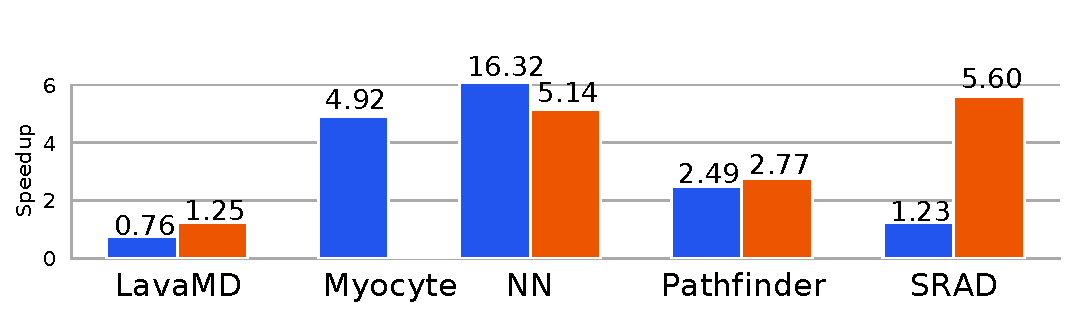
\includegraphics[width=1\linewidth]{Figures/speedup1.pdf}
  \end{center}

\end{frame}


\subsection{Status, Perspective, Strategy and Research Directions}

\begin{frame}[fragile,t]
   \frametitle{Current Status of Futhark}

\blue{Academic Perspective:}\smallskip
\begin{itemize}
    \item been playing catch-up with academic competitors\\ 
            with rather limited resources (1 PhD, couple of MSc)\smallskip
        \begin{itemize}
            \item reached ``state of the art'' level (TACO'17, PLDI'17, ICFP'18?),
            \item relatively mature framework, suitable for building on top of it,
            \item new research directions (later); focus on code transformations.
        \end{itemize}\smallskip
    \item solid foundation \& vehicle for conducting research in system's area.
\end{itemize}
\bigskip

\blue{Funding Perspective:} languages/compilers subsidized. Selling points:\smallskip
\begin{itemize}
    \item natural expression of algorithms + modularity + composibility; \smallskip
    \item generate efficient code for capricious modern hardware (GPUs); \smallskip
    \item integration with mainstream productivity environments;\smallskip
    \item one of the main outcomes of HIPERFIT project.
\end{itemize}

\end{frame}

\begin{frame}[fragile,t]
   \frametitle{Strategy}

\blue{Languages/compilers are subsidized everywhere ... What to do?}
\bigskip

\emphh{Invest(ed) a lot of effort on getting Futhark used:}\smallskip
\begin{itemize}
    \item ongoing collaborations: SimCorp,~LexiFi,~3Shape,~BK~Medical,~ESS,~Dyalog
    \begin{itemize}
        \item industrial PhD with SimCorp (Cosmin + Martin)
        \item hope for an industrial post-doc with SimCorp \& LexiFi\smallskip
    \end{itemize}
    \item some collaboration with The Image group; potential for more\smallskip
    \item Futhark used in two MSc courses + several MSc thesis.
\end{itemize}
\bigskip

\emphh{Build potential for collaboration with academic partners:}
\begin{itemize}
    \item invited talks, conference participation, students internships;
    \item visibility: PC work (vice-chair IPDPS'18, co-chair FHPC'17, PACT, PPoPP, ISC);
    \item collaborative frameworks; gather support for research agenda
\end{itemize} 

\end{frame}


\begin{frame}[fragile,t]
   \frametitle{Several Future Research Directions}

\blue{Ultimate goal: tough to beat the compiler by 
    programming assembly.}

\begin{itemize}
    \item \emphh{Dataset-Sensitive Compilation (DSC)}
        \begin{itemize}
            \item intuition: outer parallelism typically more profitable
            \item incremental utilization of parallelism (top-down)
            \item multi-versioned code discriminated by
                    statically inferred predicates,
                    whose threshold values are autotuned +
                    %to hardware specifics +
            \item reordering optimisations by inspector-executor
                    techniques;
        \end{itemize}\medskip\pause

    \item \emphh{Statically-Inferred Memory Management (MEM):}
        %frees the programmer from worrying about memory management;
        %responsibility shifted to compiler:
        \begin{itemize}
                    \item build on region-based memory management for
                            introducing a notion of memory into a
                            memory-agnostic program +
                    \item lift the semantics of register allocation
                            and coalescing to operate on arrays,
                            rather than scalars.
        \end{itemize}\medskip\pause

    \item \emphh{Language Extensions:}
        \begin{itemize}
            \item support for other bulk datatypes, e.g.,
                    multisets for SQL queries
            \item support for expressing, reasoning and optimising
                    (multi)linear functions,
                    e.g., automatic differentiation
        \end{itemize}
    \medskip
    \item \emphh{Transition towards ``real'' HPC (clusters of GPU/FPGA)}
\end{itemize}
\end{frame}

\begin{frame}[fragile,t]
   \frametitle{Several Future Research Directions (cont)}

\begin{itemize}
    \item ``FUTHARK: Functional Technology for High-performance Architectures'',
    FTP18 grant proposal (Fritz, Martin, Ken, Cosmin).\bigskip

    \item Strong support from industry and academic partners:\smallskip
    \begin{itemize}
        \item industry: SimCorp, LexiFi, 3Shape, Dyalog, BK Medical, NVIDIA, MSR, LLNL\smallskip
        \item academy:  Kevin Hammond, Vinod Grover, Ranjid Jhala, Simon Peyton Jones, 
                Gabriele Keller, Paul Kelly, Alan Mycroft, Jens Palsberg, Olga Pearce, 
                Lawrence Rauchwerger, P. Sadayappan, Phil Trinder, and Dimitrios Vytiniotis.
    \end{itemize}\bigskip

    \item build consortium for EU projects, above + Albert Cohen, Mary Sheeran, Per Stenström.
\end{itemize}

\end{frame}

\end{document}
